\documentclass[12pt,parskip=full]{article}
\usepackage{lmodern}
\usepackage{amsmath}
\usepackage[left=1.0in,right=1.0in,top=1.0in,bottom=1.0in]{geometry}
\geometry{letterpaper}
\usepackage{graphicx}
\usepackage{caption}
\usepackage{subcaption}
\usepackage{longtable}
\usepackage{float}
\usepackage{wrapfig}
\usepackage{soul}
\usepackage{textcomp}
\usepackage{marvosym}
\usepackage{wasysym}
\usepackage{latexsym}
\usepackage{amssymb}
\usepackage{apacite}
\usepackage{tabu}
\usepackage[svgnames]{xcolor}
\usepackage{tikz}
\usepackage[linktoc=all]{hyperref}
\usepackage{cleveref}
\usepackage{listings}
\usepackage{setspace}
\usepackage{parskip}
\usepackage{array}
\usepackage{apacite}
\usepackage{natbib}
\usepackage{multicol}
\usepackage{subcaption}
\usetikzlibrary{arrows}

\pgfdeclarelayer{edgelayer}
\pgfdeclarelayer{nodelayer}
\pgfsetlayers{edgelayer,nodelayer,main}

\tikzstyle{none}=[inner sep=0pt]
\tikzstyle{waypt}=[circle,fill=Black,draw=Black,scale=0.4]
\tikzstyle{Helobody}=[circle,fill=White,draw=Black,scale=4.0]
\tikzstyle{Tailrotor}=[circle,fill=White,draw=Black,scale=1.0]
\tikzstyle{ForceVector}=[->,draw=Indigo,fill=Indigo]
\tikzstyle{Coordinate}=[->,draw=Red,fill=Red,fill opacity=1.0]
\tikzstyle{angle}=[->]
\tikzstyle{MeasureMark}=[|-|]
\newlength{\imagewidth}
\newlength{\imagescale}

\setlength{\parskip}{11pt}
%\setlength{\parindent}{15pt}
\usepackage{bookmark}
\makeatletter
\renewcommand\@seccntformat[1]{}
\makeatother

\lstset
{
    language=Matlab,
    keywords={break,case,catch,continue,else,elseif,end,for,function,
        global,if,otherwise,persistent,return,switch,try,while},
    basicstyle=\ttfamily,
    keywordstyle=\color{blue},
    commentstyle=\color{ForestGreen},
    stringstyle=\color{purple},
    numbers=left,
    numberstyle=\tiny\color{gray},
    stepnumber=1,
    numbersep=10pt,
    backgroundcolor=\color{white},
    tabsize=4,
    showspaces=false,
    showstringspaces=false
}

\renewcommand{\thesection}{\arabic{section}}

\renewcommand{\thesubsection}{\thesection\alph{subsection}}
\renewcommand{\theequation}{\thesubsection\arabic{equation}}

\numberwithin{subsection}{section}

\begin{document}
	\vspace{-2ex}
	\title{Report 1: Line Search\vspace{-3.5ex}}
	\author{Rob Rau\vspace{-4ex}}
	\date{\today\vspace{-4ex}}
	\maketitle
	
	
	\section{Introduction}
	
		Two different line search methods were used to optimize the simple drag coefficient equation
		\begin{equation}\label{eqn:cd1}
			C_D = kC_f \frac{S_w}{S} + \frac{C_{L}^2}{\pi AR e}
		\end{equation}

		Where $k$ is the form factor that accounts for pressure drag, $C_f$ is the skin friction coefficient, $S_w$ is the wetted surface
		area of the aircraft, $S$ is the reference planform area, $C_L$ is the lift coefficient, $AR$ is the aspect ratio, and $e$ is the
		Oswald span efficiency factor. This equation can be modified to be written in terms of $AR$ using the following relations
		\begin{eqnarray}
			C_f = \frac{0.074}{Re} \\
			Re = \frac{\rho V c}{\mu}
		\end{eqnarray}
		Where $Re$ is the Reynolds number, $V$ is the aircraft velocity, and $c$ is some characteristic length that the flow follows, in
		this case, the chord of the wing. The aspect ratio is non-dimensional number that is expressed in terms of the wing span $b$ and
		and reference planform area.
		\begin{equation}
			AR = \frac{b^2}{S}
		\end{equation}
		With these relations and by holding the values of $V$, $S$, $S_w$, $\rho$, $\mu$, $k$, and $e$ constant \cref{eqn:cd1} can be
		written as a function the aspect ratio.
		\begin{equation}
			C_D = k \frac{0.074}{\left(\frac{\rho V S \sqrt{S AR}}{\mu} \right)^{0.2}} \frac{S_w}{S} + \frac{C_{L}^2}{\pi AR e}
		\end{equation}
		The goal of the optimizer is to find the aspect ratio, that gives the lowest drag.

		Both optimizers were ran in a number of different test cases. Each test case had a different starting point and interval
		in order to observe how these parameters affect convergence and to compare the two optimizers.
		
		The golden section search works by taking an interval and initial point and reduces the interval until an optimal solution is
		found. The interior points of the interval are chosen in such a way that when the interval is reduced, only one more function
		evaluation is needed before reducing again.
		
		The final optimized value is an aspect ratio of 28.3818 with a drag coefficient of 0.0115725.

	\section{Convergence}
	
		Both the golden section search and the bracket and zoom algorithm exhibit linear convergence. However, the bracket and zoom algorithm
		has a higher rate of convergence as seen in \cref{fig:convergence}.
		
		\begin{figure}[h]
			\centering
			\begin{subfigure}[h]{0.45\textwidth}
				\includegraphics[width=\textwidth, angle=270]{Convergance_1_40.eps}
				\vspace{-13ex}
				\subcaption{Initial point: 1, Interval: 40}
			\end{subfigure}
			\begin{subfigure}[h]{0.45\textwidth}
				\includegraphics[width=\textwidth, angle=270]{Convergance_1_65.eps}
				\vspace{-13ex}
				\subcaption{Initial point: 1, Interval: 65}
			\end{subfigure}
			\begin{subfigure}[h]{0.45\textwidth}
				\includegraphics[width=\textwidth, angle=270]{Convergance_10_20.eps}
				\vspace{-13ex}
				\subcaption{Initial point: 10, Interval: 20}
			\end{subfigure}
			\begin{subfigure}[h]{0.45\textwidth}
				\includegraphics[width=\textwidth, angle=270]{Convergance_20_90.eps}
				\vspace{-13ex}
				\subcaption{Initial point: 20, Interval: 90}
			\end{subfigure}
			\caption{Comparison of convergence rates for the golden section search (red) and the bracket and zoom algorithm (blue)\label{fig:convergence}}
		\end{figure}
		
		This general trend seems to be independent of start point and interval. I did not have enough time to compute the exact convergence rate.
	\section{Performance}
		
		Even though the bracket and zoom algorithm has a slightly higher convergence rate, it consumes more computation time per iteration than the golden
		section search. The golden section search, on average, consume 1.35 micro seconds of cpu time per iteration where the bracket and zoom 
		algorithm takes about 1.5 micro seconds per iteration. These test were tested using optimization level 3.
		
		While both algorithms only require one function evaluation the bracket and zoom 
		algorithm requires more conditional logic. Logical statements requires branching on the CPU. Moving between execution branches can be more costly 
		than just mathematical statements alone. This branching problem can be exacerbated if there is no regular pattern in the way the program branches
		thus fooling the CPU's branch predictor, and generating cache misses. Cache misses can severely slow down code execution. This is only a potential
		issue, and not what I think is happening in this case, but a cautionary tail none the less. In comparison the golden section search has far 
		fewer conditionals and is more mathematical in nature.
		
		It would be interesting to try this code with a different compiler and see if there are any performance differences. The GNU implementation
		of the D Programming language could benefit from the mature backend code generation optimizations.
		
	\section{Other Thoughts and Observations}
	
		Starting each algorithm at different points and using different intervals brought a few things to my attention. The golden section search is
		limited by the start point and the interval given to it. It cannot decide in which direction to apply that interval, so if the start point is
		past the optimal point, it will converge on the best local minimum in the interval. The bracket and zoom algorithm doesn't have this problem
		as it computes the gradient to chose which direction to apply the search interval.
		
		Although it is obvious now, I had thought I had a bug in my bracket and zoom algorithm when running case that started past the physically optimal
		point, and had a large interval. The optimizer was reporting a negative optimal aspect ratio. This puzzled me until I realized that the drag 
		coefficient was indeed lower at the non-physical solution. This is why constraints will be added later.
		
	\section{Code}
	
		The algorithms as they are right now do not support multiple design variables, but the way the underlying framework has been built makes it trivial
		to extend this functionality. The base objects and interfaces in the Multidisciplinary Design and Optimization Library (MDOL) are all built to 
		support multiple design variables so the only changes that need to be made are in the specific implementations.
		
		So far the choice of the D Programming language has led to very clean code and an easy to understand and extensible framework. 
		This isn't to say there have been no learning curves or unforeseen issues. When implementing the complex step to use the bracket and zoom algorithm,
		I was testing it on the test polynomial seen in the notes
		\begin{equation}
			f(x) = (x - 3)x^3(x-6)^4
		\end{equation}
		it would incorrectly compute the derivative at certain points. I found that when the step size was set to small ($< 10e-10$), the $(x-6)^4$ portion 
		of the equation would have error in the imaginary portion. Setting the step size to $10e-10$ fixed this, but I will be continually verifying this
		to be sure.

\end{document}
